\chapter{Design}
To address the requirements presented in \cref{chap:requirements}, we developed a system composed of several components, as illustrated in \cref{fig:baseArchDiag}
and more in detail in \cref{fig:fullArchDiag}:
\begin{itemize}
    \item A set of \textit{smart contracts} responsible for all blockchain-related operations, including \acrshort{sw} creation and transaction management.
    \item A \textit{browser extension} that allows students to manage their academic wallets.
    \item A \textit{\acrfull{sdk}} designed for universities to interact with the \acrshort{ew} system.
    \item An external \textit{decentralized storage system} used to store and retrieve certification files (see \cref{sec:decStorageDesgn}).
\end{itemize}
\begin{figure}[htpb]
  \centering
  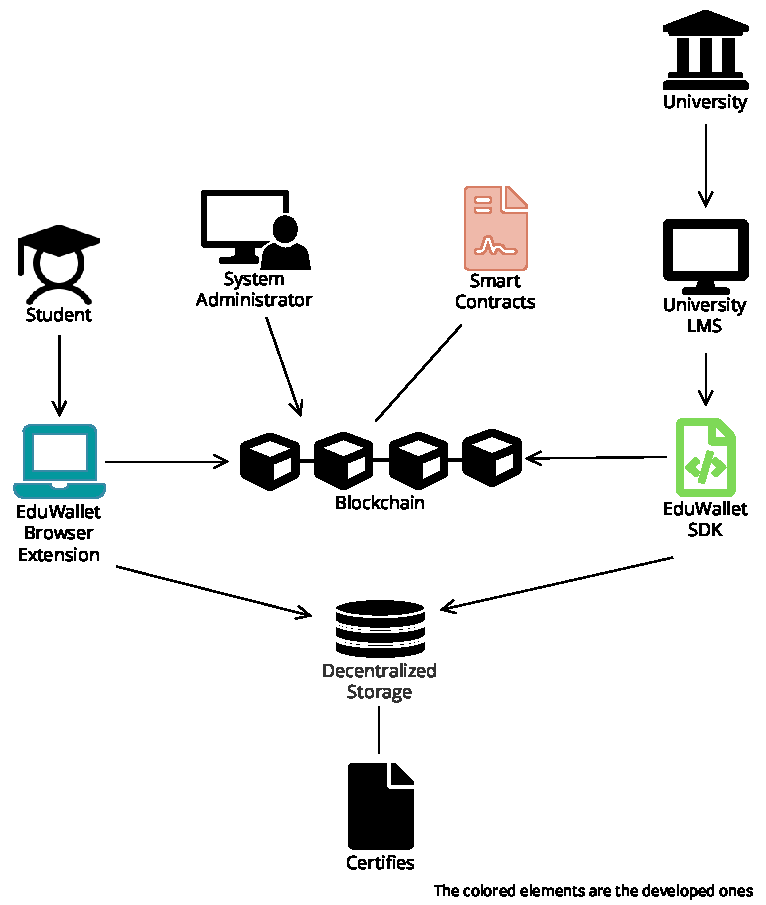
\includegraphics[width=0.5\textwidth]{figures/Architecture diagram basic.pdf}
  \caption[System basic architecture diagram]{The diagram shows the base architecture of the \acrlong{ew} system.}
  \label{fig:baseArchDiag}
\end{figure}

In addition to these core components, we developed a simple yet complete \textit{\acrfull{cli}}, which simulates a university's \acrshort{lms} and its interaction with the academic records system. The \acrshort{cli} serves as a testing and demonstration tool and enables users to perform all operations typically available to universities, thereby simplifying the interaction with our \acrshort{sdk}.

Since the focus of our work is on the interaction of universities and students with the academic registry, the system administrator's core functionality\footnote{The approval and subscription of universities} have been inserted directly in the \acrshort{cli}. This design decision streamlines our use case and reduces unnecessary complexity.

A more detailed analysis of each component is provided in the following sections.

\begin{figure}[htpb]
  \centering
  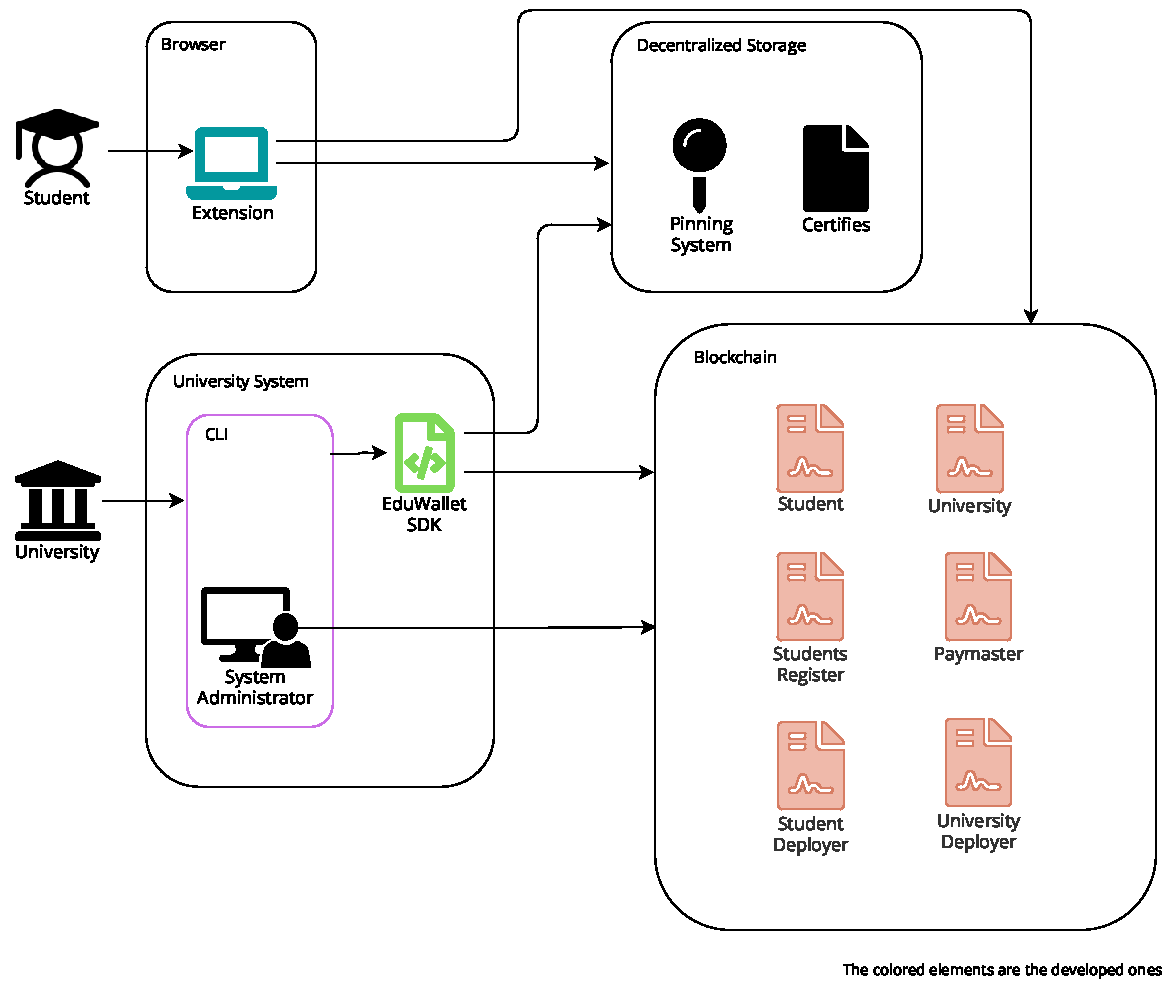
\includegraphics[width=0.7\textwidth]{figures/Architecture diagram complete.pdf}
  \caption[System architecture diagram]{The diagram shows the entire architecture of the \acrlong{ew} system.}
  \label{fig:fullArchDiag}
\end{figure}

\section{Smart Contracts}
\label{sec:smartContractsDesign}

\section{Browser Extension}
\label{sec:browserExtensionDesign}

\section{Decentralized Storage System}
\label{sec:decStorageDesgn}
To overcome one of the most significant challenges in blockchain systems, the cost of on-chain storage, we introduce an off-chain decentralized storage solution in our project. This system is used to store and retrieve certification files, such as language certificates or graduation diplomas, which require significantly more space than plain text\footnote{PDF files typically range from a few kilobytes to several megabytes, whereas plain text data usually occupies only a few bytes.}. Storing such documents directly on-chain would result in substantial gas costs, making the approach impractical. 

\subsection{Why a decentralized storage?}
We chose a decentralized storage system over traditional local or cloud-based solutions to maintain the decentralized nature of our environment and to meet the non-functional requirements outlined in \cref{sec:nonFunctionalRequirements}. Among the various decentralized options available, we selected \acrfull{ipfs} for its ability to provide verifiable and distributed file storage. This choice is motivated by several factors: \acrshort{ipfs} is an open source protocol with a large and active community, strong support, and widespread adoption. It also serves as the foundational layer for many other decentralized platforms, such as Filecoin\footnote{\url{https://filecoin.io}} and Web3.Storage\footnote{\url{https://web3.storage}}, allowing future extensions or upgrades to be implemented with minimal effort \cite{erikflorian2022ipfsandfrineds}. Furthermore, \acrshort{ipfs} ensures immutability of stored files, a critical feature for academic certificates, which must remain unchanged over time.

\subsection{Pinning files}
To fully leverage \acrshort{ipfs}, we integrated Filebase\footnote{\url{https://filebase.com}}, a third-party pinning service. Pinning refers to the act of instructing a node to keep a copy of a file permanently, preventing it from being removed during garbage collection. Without Filebase, we would have needed to run our own local \acrshort{ipfs} node and manage file pinning manually, an approach that introduces instead complexity, higher maintenance costs, and reduced data availability in a testing system like ours. In contrast, Filebase handles node operation and file pinning, offering an accessible solution thorough its AWS S3-compatible \acrshort{api}, which simplifies file uploads to the peer-to-peer network. Notably, Filebase also provides a free tier allowing up to 5 GB of storage, which is sufficient for our needs. This is an advantage over other pinning solutions such as Web3.Storage, which lacks a fully free plan, or Pinata\footnote{\url{https://pinata.cloud}}, which offers more limited options.

\subsection{Integration in the system}
As shown in \cref{fig:fullArchDiag}, both the browser extension and the \acrshort{sdk} interact with the storage system. The browser extension retrieves certificate associated with academic records using the official \acrshort{ipfs} public gateway. It presents students with a direct link to each certificate, composed by the gateway's base \acrshort{url} followed by the file's \acrfull{cid} on the \acrshort{ipfs} network. The \acrshort{cid} of each document is stored on-chain within the student's academic wallet, alongside other record information such as the course name. This enables students to view and download their certificates from a standard web interface.

% TODO: Add photo of the extension where you can see the link of a certification
Similarly, the \acrshort{sdk} uses the same mechanism to retrieve certificates on behalf of universities. When uploading a file, however, the \acrshort{sdk} interacts directly with Filebase to ensure the file is pinned and hosted by an active node. The \acrshort{sdk} receives the document from the university, then uses the AWS S3-compatible \acrshort{api} to upload it. The \acrshort{api} requires the key associated with the pinning account (managed by the \acrshort{ew} system administrator) and the file itself. In return, it provides the \acrshort{cid}, which is then stored in the academic record.
% TODO: Reference implementation section

\subsection{Security and Limitations}
Academic certifies, and official documents more broadly, are legal artifacts that must always be secure and verifiable. \acrshort{ipfs} inherently supports these properties through its use of content-based addressing. In this model, each file is identified by a \acrshort{cid}, which is derived from the cryptographic hash of the file's content. Any alteration to the file results in a completely different \acrshort{cid}, ensuring that tampering is immediately detectable \cite{benet2014ipfscontentaddressed}. Since the the \acrshort{cid} is stored on the blockchain at the time the certificate is issued by the university, the document's authenticity and integrity are guaranteed.

While \acrshort{ipfs} offers strong immutability and verifiability, it lacks built-in access control. In the context of our system, we assume that certificates are publicly accessible documents. Consequently, any part in possession of a file's \acrshort{cid} can retrieve it via the public gateway. However, if access control becomes a requirement, there are several strategies to address this limitation \cite{barbaraanrealaura2021datapersistence}. One option is to encrypt files before uploading them to \acrshort{ipfs}, such that only authorized components within our system can decrypt them. Another approach is to use a private \acrshort{ipfs} network, where access can be restricted to approved entities. The trade-offs and potential implications of such private deployment will be discussed in the FUTURE WORK CHAPTER.

\section{\acrshort{cli}}
\label{sec:cliDesign}